If we are to be able to estimate the trajectories based on the initial conditions successfully, we
need to be able to reliably solve the forward problem\footnote{See section \ref{inverse} for a definition
of a forward problem.} for the trajectory of the golf ball. In order
to do this, as stated at the end of the previous chapter, we must find an improved form for $c_D$ which
more accurately describes the physics which occurs during the flight of a ball.

There are a number of approaches to this, and we have attempted a few of them in our investigations
in an attempt to find which of them gives the most reliable results. Any model of golf ball flight which
captures the dynamics of an individual ball will have to use flight data to inform the exact parameters
in a drag function for that ball. Thus, much of this chapter is also concerned with attempting to find 
methods of estimating the parameters for such functions given data on the flight of a particular ball.

This parameter estimation is an example of an inverse problem. Some generalities on such problems are
given in the appendix.

\section{Estimating $c_{D}$ from Experiments}

As a first attempt at estmiating $c_D$, we began by returning to the form given in \citet{Morrison2010}
and discussed in section \ref{sec:drag-crisis}. Recalling that we expect the dimpled surface of the
golf ball to have the affect of moving the point at which the drag crisis occurs to lower Reynolds
numbers, we began by taking Morrison's form for the drag and attempting to change the coefficents to
``move'' the drop in drag to within the range seen within experiments on golf balls.

Here, we attempt to match the function to the experimental data given in various papers which we
have listed before. After some consideration, the following form of $c_D$ can be found to fit
with a number of different experiments

\begin{equation} \label{drag-m-mod}
c_D = \frac{24}{Re} + \frac{2.6(Re/5)}{1 + (Re/5)^{1.52}} + \frac{0.38(Re/121000)^{-7.94}}{1+(Re/121000)^{-8.00}}
+ \frac{Re^{0.83}}{450000} .
\end{equation}

We believe that this form captures the physics we expect to see from the golf ball better than simply
taking a constant value of $c_D$ as in \citet{Robinson2013}. Plotting the original and the modified
form of $c_D$ shows how the drag has moved to within the range we expect to see.
\begin{figure}
% In folder Morrison
\centering
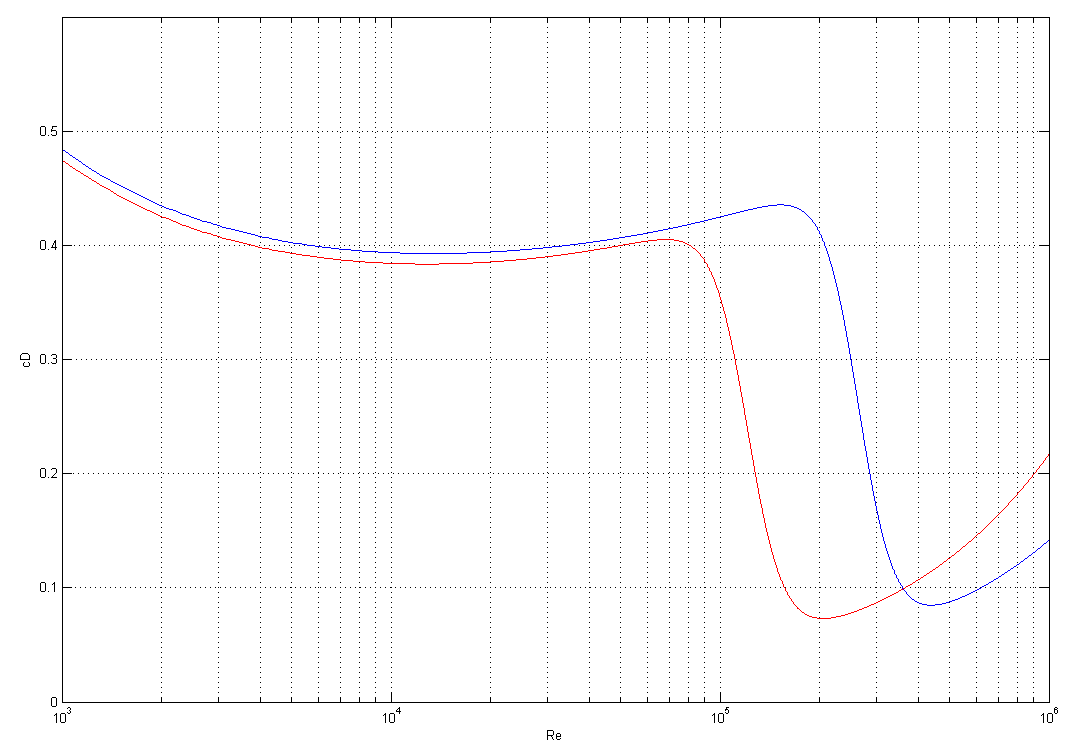
\includegraphics[scale=0.55]{../images/morrison-modified.png}
\caption[Plotting the original Morrison form against a modified version for golf balls]{In blue is the
original $c_D$ function, given in \eqref{drag-m}. In red is the modified form, \eqref{drag-m-mod}, which
takes into account the lower value of Reynolds number where the transition to lower drag occurs.}
\end{figure}

This form has a number of limitations, but does serve to be a good initial start at working out the 
drag for a golf ball. The weaknesses can be summarised as
\begin{itemize}
\item This form of $c_D$ is constant for all types of golf balls, which we know is not the case for
realistic balls, as noted in \citet{Alam2011}.
\item Changing this function for different balls is a matter of hand choosing coefficents in the terms
of \eqref{drag-m-mod}. This method is not at all easy to modify for other balls.
\item While the form of $c_D$ is dimensionless, as we require it to be, there is no dependence on spin
at all, which could be causing significant contributions to the drag.
\end{itemize}

Replacing $c_D$ in the model by Robinson and Robinson by $c_D$ as defined in \eqref{drag-m-mod} does
make a significant change to the resultant trajectory, bringing the height of the ball much closer to
the experimental trajectories and improving the carry of the ball significantly.

% \begin{itemize}
% \item We try to find results for spheres and change them to account for the earlier drag crisis.
% \item Take the function from \citet{Morrison2010} and change the coefficents to ``move'' the drag 
% drop to lower values of $Re$.
% \item This works fairly well but cannot capture all of the behaviour, as other work shows that
% different balls should expect to see different drags \citet{Alam2011}.
% \end{itemize}

\begin{figure}[h]
\centering
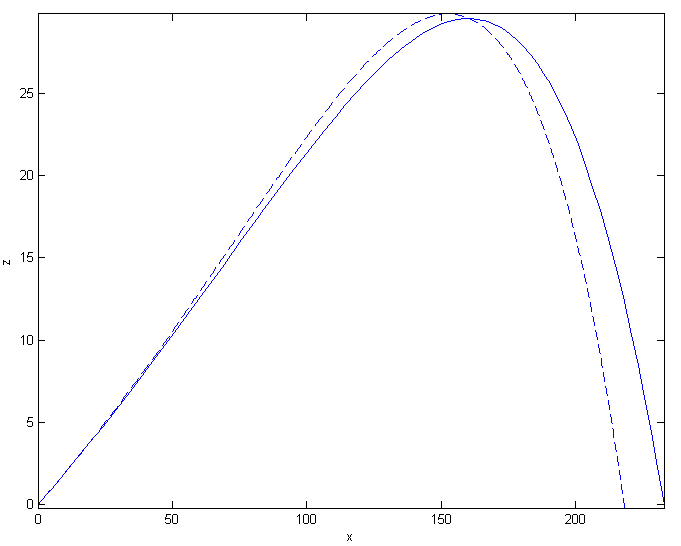
\includegraphics[scale=0.8]{../images/m-mod-data1.png}
\caption[Model with using the modified Morrison form for $c_D$.]{Using the modified Morrison form for $c_{D}$ results 
in a fairly accurate profile. Here the solid line is the model prediction 
and the dashed line is the data.}
\label{m-mod-data1}
\end{figure}

In Figure \ref{m-mod-data1} we see that this form of the drag function brings the model and experimental
results into close agreement with each other. However, viewing the trajectory in 3D reveals that while
the height and carry of the ball are predicted well, the motion along the $y$ axis is not predicted
as well, deviating by approximately $5$m at the end of the trajectory.

\begin{figure}[h]
\centering
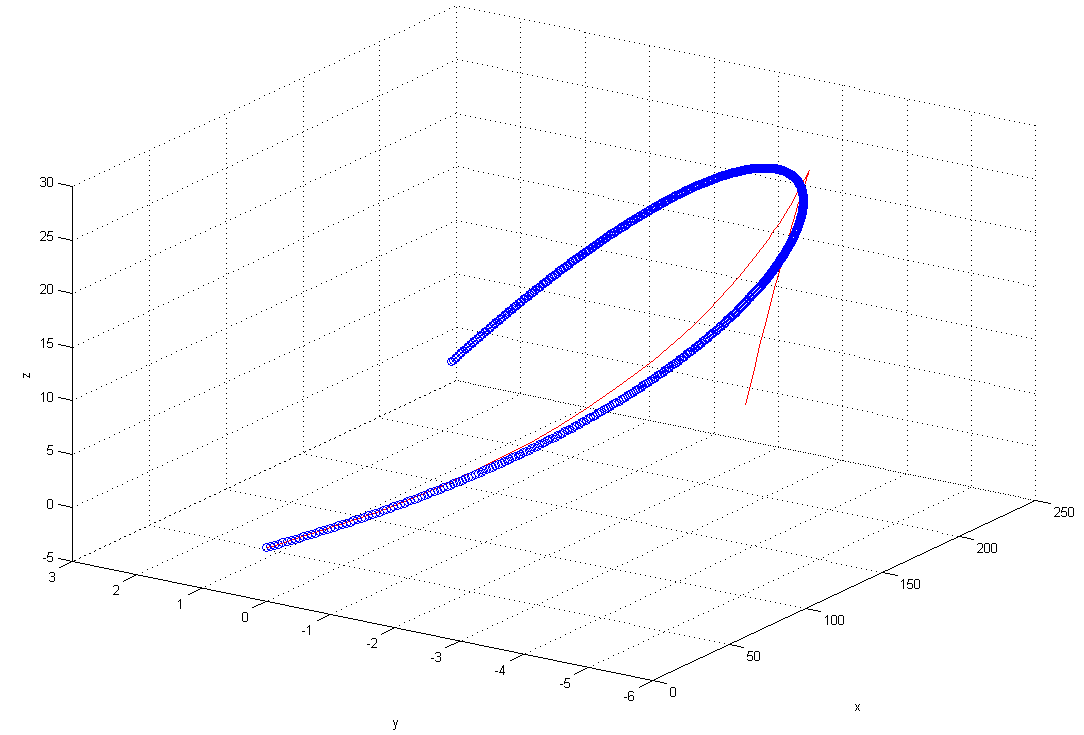
\includegraphics[scale=0.5]{../images/m-mod-data1-3d.png}
\caption[Model with using the modified Morrison form for $c_D$ in 3D.]{This is a 3D plot of Figure \ref{m-mod-data1}.
We note that initially the predicted curve fits the data almost perfectly, being within 1m. Just before
the apex of the curve however the data (plotted with circles) veers back towards the $y=0$ line, whereas
the model (in red) does not have this behaviour.}
\end{figure}

While we see good agreement between the model and the data for this data set, running the model with
a different set of initial conditions and using data taken with a different ball does not yeild such
close agreement.

The R\&A provided another data set, this time with 4 trajectories using the same ball. If we select
the second trajectory from this data set to test to test this model against, with the following 
initial conditions
\[
x = -0.112, \,\, y = 0.024, \,\, z = 0, \,\, v_x = 69.438, \,\, v_z = 9.247, \,\, v_y = -0.633, \,\,
|\vec{\omega}| = 370.71,\,\, \theta = \frac{167\pi}{180} .
\]
we find (see Figure \ref{data2-2d}) that the trajectory does not match as closely as the previous data.

This is not that surprinsing however: the two separate data sets are using different balls, and thus
we would expect the $c_D$ to change between the two balls.

While the modified Morrison form does give better results than simply taking $c_D$ to be constant
it cannot possibly explain how $c_D$ varies for every ball. However, seeing that this form of the drag
brings the model much closer in line with experimental data is encouraging, and implies that factoring
in the drag crisis to the calculation of the model does have a major effect on the resultant trajectories
as we expected it to do so.

\begin{figure}
\centering
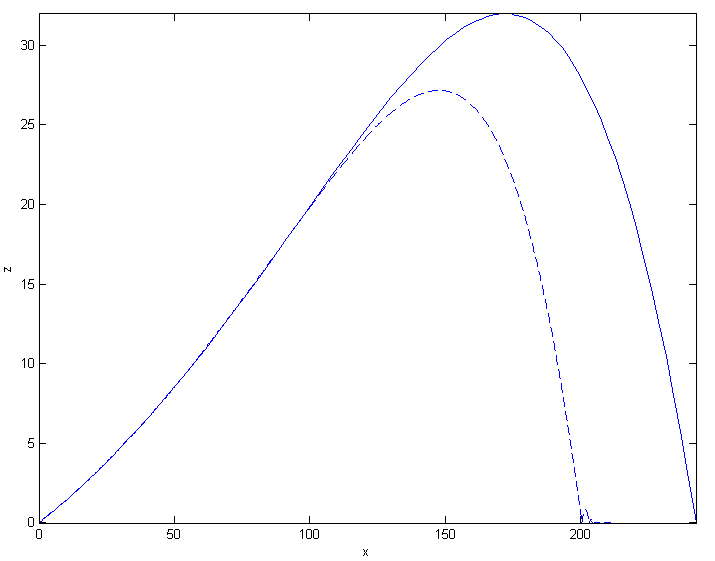
\includegraphics[scale=0.8]{../images/data2-2d.png}
\caption[Second data set using the modified Morrison form.]{Here the dashed line is the second data
set and the solid line is the model using the modified Morrison form.}
\label{data2-2d}
\end{figure}

\section{Parameterising $c_{D}$ and $c_{L}$ by Non Dimensional Variables}

We now attempted a different approach: following the idea of \citet{Lieberman2001} we attempted to
use the data from The R\&A to estimate parameters in functions of dimensionless groupings for $c_D$
and $c_L$. 

\citet{Lieberman2001} give a number of forms for $c_D$ and $c_L$. We will use the first form given in
the patent, that is
\begin{subequations}
\begin{align}
c_D &= \bar{A} + \bar{B} Sr^2 + \bar{C} Re + \bar{D} Sr \\
\shortintertext{and}
c_L &= \hat{A} + \hat{B} Sr + \hat{C} Re^{-2} + \hat{D} Sr^2
\end{align}
\end{subequations}
where $Re$ is the Reynolds number as before, and $Sr$ is the spin ratio, defined as
\[
Sr = \frac{|\vec{\omega}|D}{v} .
\]
The spin ratio another possible dimensionless grouping, which emerges when performing the same analysis
as section \ref{sec:drag} but with $\omega$ and $\theta$ as part of the analysis. $D$ is the diameter
of the golf ball.

The coefficents $\bar{A}, \bar{B}, \bar{C}, \bar{D}, \hat{A}, \hat{B}, \hat{C}, \hat{D}$ are to be
determined using the data. In order to do this, we use a non linear least squares method (see appendix 
\ref{ls}) to fit the parameters within the model to the data set at hand.

In order to solve the problem we must specify an initial guess for the coefficents, before allowing
the least squares algorithm to refine the parameters. The values for the guesses were found by 
simply hand optimizing the functions based on typical speeds and spins for golf balls, changing the
coefficents until the values of $c_D$ and $c_L$ became fairly close to the values we expect them to
take from experiments.

For $c_D$ we take
\[
\bar{A} = \bar{B} = \bar{C} = \bar{D} = 6 \times 10^{-6}
\]
and for $c_L$ we take
\[
\hat{A} = \hat{B} = \hat{C} = \hat{D} = 0.5
\]
as the initial guesses.

Running these against the data provided by The R\&A provides mixed results. For some trajectories, 
the fit is almost perfect in all three dimensions as we see in Figure~\ref{ls-data2-1-2d} and 
Figure~\ref{ls-data2-1-3d}. However,
when using the same ball with different initial conditions we sometimes obtain worse fits, which do not match
as well as the previous data set, for example Figure~\ref{ls-data2-3-2d}. For some of the data sets
the least squares algorithm with the guesses as above cannot fit the data at all, as the new values 
of the parameters estimated render the equations of motion impossible to integrate using the standard routines within
MATLAB and the guesses must be changed to proceed with this data set. This implies that the model
is incredibly sensative to the choice of initial conditions 

Additionally, when comparing the 

\begin{figure}
\centering
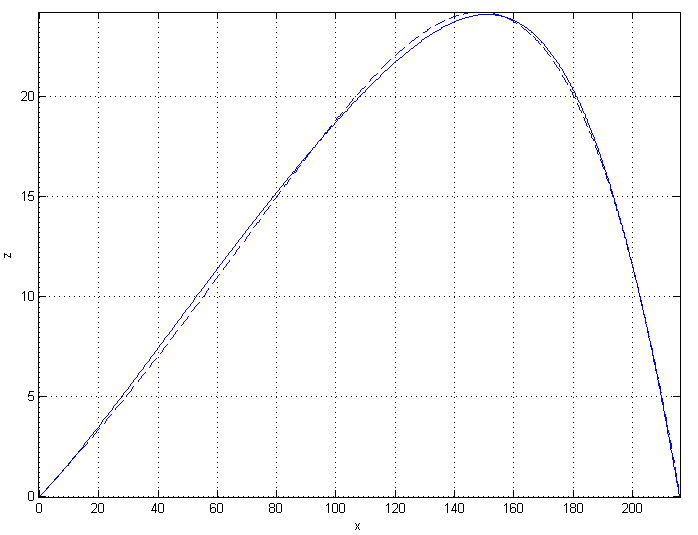
\includegraphics[scale=0.7]{../images/ls-data2-1-2d.png}
\caption[Least squares using the Re and Sr form on data]{Here we plot the least squares fit using
the $c_D$ and $c_L$ from \citet{Lieberman2001} in solid line against the data set it was fitted to
in dashed line.}
\label{ls-data2-1-2d}
\end{figure}

\begin{figure}
\centering
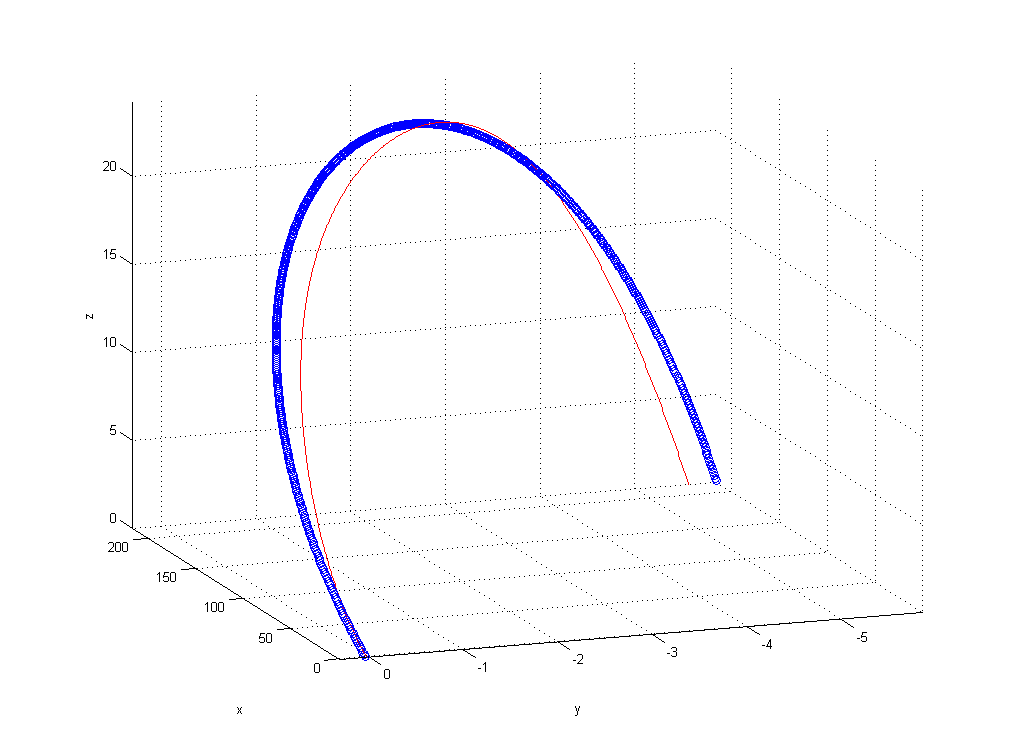
\includegraphics[scale=0.55]{../images/ls-data2-1-3d.png}
\caption[Least squares using the Re and Sr form on data in 3D]{Here we plot the data and trajectory from
Figure~\ref{ls-data2-1-2d} in 3D. Note how close the red model curve has almost identical carry and shape to the thick blue data points.}
\label{ls-data2-1-3d}
\end{figure}

\begin{figure}
\centering
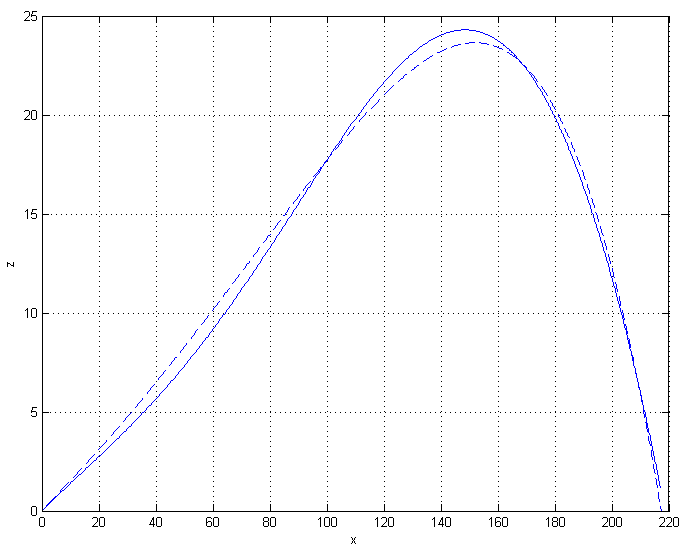
\includegraphics[scale=0.6]{../images/ls-data2-3-2d.png}
\caption[Trajectory which least squares struggles to fit]{Attempting to fit the $c_D$ and $c_L$ from
\citet{Lieberman2001} works slightly less well for this trajectory than for Figure~\ref{ls-data2-1-2d}.}
\label{ls-data2-3-2d}
\end{figure}

% \begin{itemize}
% \item We follow the idea from \citet{Lieberman2001}: form $c_{D}$ and $c_{L}$ from dimensionless
% groupings and use the data to estimate the parameters in this model.
% \item Use least squares to do this. See Appendix for discussion of what an inverse problem is, how
% to use least squares to solve them, and what numerical techniques there are to do this.
% \item Find that doing this is very hard: the problem is likely not well posed and finding a minimum
% is difficult. Would benefit from a more through analysis of the least squares problem but unsure how
% this would be done.
% \item This inverse problem is a good way to move forwards with the problem in the future.
% \end{itemize}

\section{$\tanh$ Matching}

\begin{itemize}
\item Take a hybrid approch between the two previous ideas: form a function which ``looks'' similar
to \citet{Morrison2010} and has the same behaviour, but is parameterised in such a way as to allow
us to use a least squares solver to estimate parameters.
\item For the drop, use a $\tanh$ function of the form
\[
c_{D} = a + b \tanh (-c(Re - d))
\]
where $a,b,c,d$ are constants which we can use least squreas to determine.
\item Match the $\tanh$ at the top with the $24/Re$ form we know from spheres and past the drop match
to the weakly linear form we see from the previous work.
\item Still trying to decide on results for this.
\end{itemize}